\section{Placing Social Contacts}
\label{sec:contacts:placing}

% TODO: split these 2 images
\begin{figure}
    \centering
    \includegraphics[width=5.5in]{images/images-06-cmyk.eps}
    \caption{Prototype interface of contact placement dimension. Life-size (left) on ground vs. Miniature (right) on a nearby surface.} 
    \label{fig:continuum:conditions}
\end{figure}

We implemented a prototype (Figure \ref{fig:continuum:conditions}) to test two conditions on the contact placement dimension, one viewing avatars in life-size, and the other viewing in miniature. 
We collected feedback from potential users during an open day at our lab as the participants tried demonstrations of the two conditions: C1-Life-sized (L) and C2-Miniature (M) representations of friend avatars. We collected feedback from 27 participants. On trying a demonstration of each condition, we asked participants to rate their experience on a 7-point Likert scale for three subjective questions on: 1) ease of use, 2) natural interaction, and 3) usefulness. We also asked participants to think of situations where it would be useful to use each condition. Then we asked them to choose one of the conditions as the best condition based on their experience. 

The results of the questions (Figure \ref{fig:continuum:results}) did not show any statistically significant data for this pilot study. However, we did notice a trend on Natural and Usefulness favouring the Miniature condition over the Life-size condition. A Wilcoxon signed-rank test showed that using Life-Sized or Miniature did not elicit a statistically significant change in ease of use ($Z=-.529, p=.597$), natural interaction ($Z=-1.616, p=.106$), nor usefulness ($Z=-1.664, p=0.096$). Participants reported the most useful scenarios for the Life-size condition as \enquote{face to face conversations with a social contact} or \enquote{when zooming in to a subset group of friends.} For the Miniature condition, participants reported \enquote{seeing the overall picture of social contacts} or \enquote{moving contacts between different social circles} as being useful. We also asked participants to rank the two conditions in terms of preference. Results (Figure \ref{fig:continuum:results}) show that more participants preferred the Miniature condition. A Wilcoxon signed-rank test showed that using Life-Sized or Miniature did not reach statistical significance ($Z=-.577, p=.564$).

\begin{figure}[ht]
    \centering
    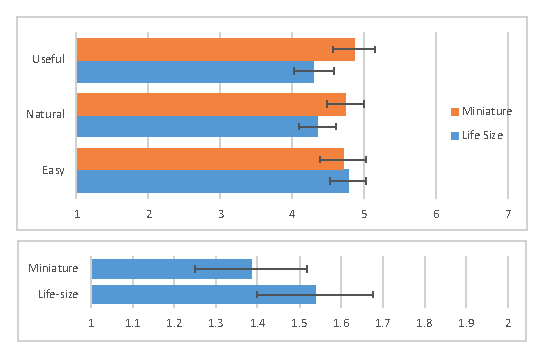
\includegraphics[width=3in]{images/images-09.eps}
    \caption{\textit{Top:} average results of subjective questions grouped by condition by question. \textit{Bottom:} average ranking results of preferred condition between Life-size and Miniature; 1=most preferred, 2=least preferred. Whiskers indicate standard error.}
    \label{fig:continuum:results}
\end{figure}